\documentclass[]{article}

%opening
\title{4F13 Probabilistic Machine Learning - Gaussian Processes}
\author{Lawrence Tray \\ St John's College}

%packages
\usepackage[margin=0.5in]{geometry}
\usepackage{graphicx}
\usepackage{amsmath}
\usepackage{amssymb}
\usepackage{hyperref}
\usepackage{caption}
\usepackage{subcaption}

%package setup
\graphicspath{{./img/}}
\DeclareMathOperator*{\argmax}{arg\,max}
\DeclareMathOperator*{\argmin}{arg\,min}

%custom commands
\newcommand{\dft}{\mathcal{F}}
\newcommand{\idft}{\mathcal{F}^{-1}}
\newcommand{\Xcal}{\mathcal{X}}
\newcommand{\Ncal}{\mathcal{N}}
\newcommand{\cmplx}{\mathbb{C}}
\newcommand{\Lcal}{\mathcal{L}}
\newcommand{\figwidth}{0.6\linewidth}

%section numbering
\renewcommand{\thesubsection}{\thesection.\alph{subsection}}

\begin{document}

\maketitle

\begin{abstract}
\end{abstract}

\section{Introduction}

\section{Questions}
\subsection{Squared Exponential Covariance Function}
We start with a simple squared exponential (SE) covariance function. As we start by working in one dimension this is necessarily isotropic. The covariance function is given by:
%
\begin{equation}
k(x, x') = \nu^2 \exp\left\{- \frac{(x-x')^2}{2l^2}\right\}
\label{eqn:covSEiso}
\end{equation}
%
The hyperparameters are $\nu$ and $l$ which control the baseline variance level and length scale of variation respectively. We load in the training data from \textit{`cw1a.mat'} and train a GP model, with zero mean and covariance function given by equation \ref{eqn:covSEiso}. We train the model by minimising the negative log marginal likelihood (denoted $\Lcal$). This optimisation yields the following change in the hyperparameters (the gpml toolbox reports log-parameters so these are included for reference):
%
\begin{alignat}{4}
\log l &: -&&1 \mapsto -2.054 ;\quad &&&l : 0.368 \mapsto 0.128 \\
\log \nu &: &&0 \mapsto -0.109  ;\quad &&&\nu : 1 \mapsto 0.897
\end{alignat}
\begin{equation}
\Lcal: 0 \mapsto -2.139
\end{equation}
%
This yields a predictor as in figure \ref{fig:1a}. The 95\% error bound is computed by $[\mu(x) - 2\sigma(x), \mu(x) + 2\sigma(x)]$. In other words, as $y \sim \Ncal(\mu(x), \sigma(x)^2)$, there is a 95\% chance of $y$ falling within two standard deviations of the mean (all evaluated at a specific $x$).
%
\begin{figure}[!h]
	\centering
	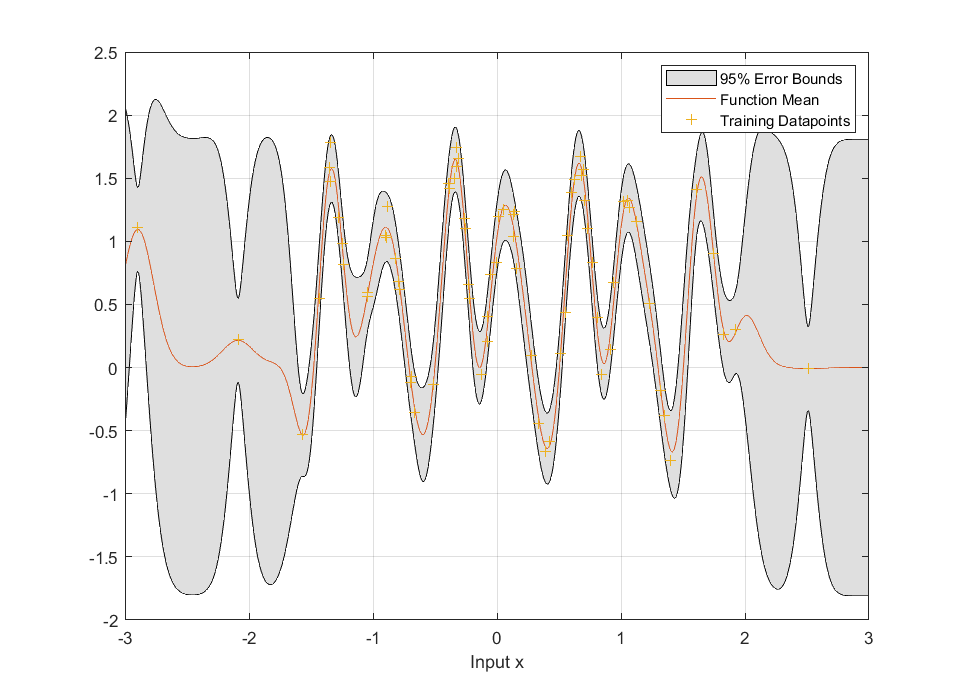
\includegraphics[width=\figwidth]{1a}
	\caption{Trained GP with initial hyperparameter settings}
	\label{fig:1a}
\end{figure}
%
We see that the error bars are always centred on the mean and that they have small standard deviations for regions in which we have many datapoints observed. This makes intuitive sense as we cannot make confident predictions in areas where the training data is sparse (such as for $|x| \geq 3$). The hyperparameters do not change enormously form the optimisation. We have that the length scale of variation $l$ shrinks slightly.
\subsection{Hyperparameter Initialisation}
\subsection{Periodic Covariance Function}
\subsection{Cholesky Decomposition}
\subsection{Model Comparison}


\end{document}
